\documentclass[11pt]{article}
\usepackage[a4paper,margin=1in]{geometry}
\usepackage{titlesec}
\usepackage{enumitem}
\usepackage{booktabs}
\usepackage{tikz}
\usetikzlibrary{arrows.meta,positioning,fit,shapes.multipart}
\pagenumbering{gobble}
\titleformat{\section}{\large\bfseries}{}{0pt}{}

\begin{document}
\section*{Technical Appendix: Query Performance at 2B Scale (ECAI)}

\textbf{Goal.} ``Find a merchant in Afghanistan selling carpets'' over a corpus of $\sim$2B facts, using \textbf{ECAI}'s SPOC$\rightarrow$curve mapping, off-chain provable indexes, and \textbf{aeternity} channels for realtime, with optional on-chain notarization.

\vspace{0.4em}
\textbf{Assumptions (realistic production):}
\begin{itemize}[leftmargin=*]
  \item Triples (\emph{Subject, Predicate, Object, Context}) deterministically map to elliptic-curve points; canonical term IDs exist for \texttt{country:AF}, \texttt{sells:Carpet}, \texttt{type:Merchant}.
  \item Inverted indexes per term use compressed bitmaps (e.g., Roaring); postings Merklized per shard; global \emph{index root} anchored to chain at regular intervals.
  \item Sharding by term-hash across 100--300 shards; queries fanned out over \textbf{aeternity state channels}; node stack in \textbf{Erlang/OTP}.
\end{itemize}

\textbf{Query plan (AND of three terms):}
\begin{enumerate}[leftmargin=*]
  \item \textbf{Normalize} to term IDs $T_{\mathrm{AF}},T_{\mathrm{Carpet}},T_{\mathrm{Merchant}}$.
  \item \textbf{Route} to shards owning those terms via channels (parallel fan-out).
  \item \textbf{Intersect} bitmaps per shard: $B(T_{\mathrm{AF}})\cap B(T_{\mathrm{Carpet}})\cap B(T_{\mathrm{Merchant}})$; return Top-K subjects + Merkle proofs.
  \item \textbf{Verify} proofs against anchored index root; optionally \textbf{notarize} answer digest on-chain via oracle (TTL).
\end{enumerate}

\begin{center}
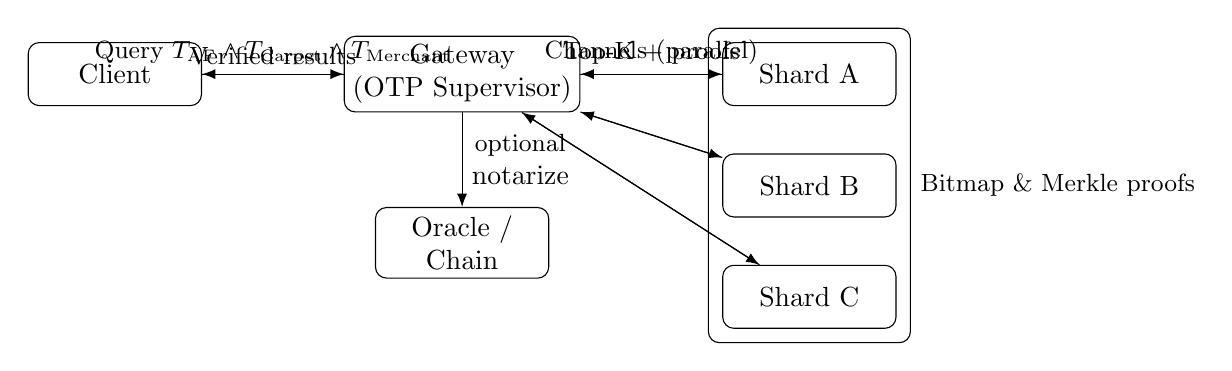
\begin{tikzpicture}[node distance=8mm]
\tikzstyle{box}=[draw,rounded corners,align=center,inner sep=3pt,minimum width=22mm,minimum height=8mm]
\node[box] (client) {Client};
\node[box,right=18mm of client] (gw) {Gateway\\(OTP Supervisor)};
\node[box,right=18mm of gw] (sh1) {Shard A};
\node[box,below=6mm of sh1] (sh2) {Shard B};
\node[box,below=6mm of sh2] (sh3) {Shard C};
\node[box,fit=(sh1)(sh3),draw,rounded corners,inner sep=5pt,label=right:{\small Bitmap \& Merkle proofs}] (cluster) {};
\node[box,below=12mm of gw] (oracle) {Oracle /\\Chain};

\draw[-{Latex}] (client)-- node[above]{\small Query $T_{\mathrm{AF}}\land T_{\mathrm{Carpet}}\land T_{\mathrm{Merchant}}$} (gw);
\draw[-{Latex}] (gw)-- node[above]{\small Channels (parallel)} (sh1);
\draw[-{Latex}] (gw)-- (sh2);
\draw[-{Latex}] (gw)-- (sh3);
\draw[-{Latex}] (sh1) -- node[above]{\small Top-K + proofs} (gw);
\draw[-{Latex}] (sh2) -- (gw);
\draw[-{Latex}] (sh3) -- (gw);
\draw[-{Latex}] (gw) -- node[right,align=center]{\small optional \\ notarize} (oracle);

\draw[-{Latex}] (gw) -- node[above]{\small Verified results} (client);
\end{tikzpicture}
\end{center}

\textbf{Latency budget (typical):}
\begin{center}
\begin{tabular}{@{}lrr@{}}
\toprule
Stage & Warm/Local & Cold/WAN \\
\midrule
Normalize terms \& route (channels) & 5--25 ms & 20--80 ms \\
Shard bitmap intersections (parallel) & 20--120 ms & 80--400 ms \\
Fan-in, Top-K, proof packing & 30--120 ms & 80--300 ms \\
Client proof verification & 5--30 ms & 10--50 ms \\
\textbf{Subtotal (realtime read)} & \textbf{60--295 ms} & \textbf{190--830 ms} \\
\midrule
Optional on-chain notarization (oracle TTL) & \multicolumn{2}{c}{\textbf{3--10 minutes} (1--2 key blocks + 1 conf)} \\
\bottomrule
\end{tabular}
\end{center}

\textbf{Why it scales on 2B:}
\begin{itemize}[leftmargin=*]
  \item High selectivity: three-term AND narrows hits dramatically.
  \item Bitmap math is word-level; intersections run per shard in parallel OTP processes.
  \item Returned proofs cover only touched postings; global integrity via anchored index root.
\end{itemize}

\textbf{Operational levers:}
\begin{itemize}[leftmargin=*]
  \item Tune shard count and postings compression; pre-compute frequent term intersections.
  \item Cache term bitmaps and Top-K heaps; keep hot shards in memory.
  \item Choose per-query: \emph{channels for realtime} vs. \emph{oracle TTL for notarized answers}.
\end{itemize}

\end{document}
